% +--------------------------------------------------------------------+
% | Sample Chapter 3
% +--------------------------------------------------------------------+

\cleardoublepage

% +--------------------------------------------------------------------+
% | Replace "This is Chapter 3" below with the title of your chapter.
% | LaTeX will automatically number the chapters.
% +--------------------------------------------------------------------+

\chapter{Examples}
\label{makereference6}

In this section we're going to explain a few use cases that could be actually applied using Epfiot application.

With these examples, a greater understanding is sought for the reader of how Epfiot works. It is also intended to serve as a guide for beginners in the use of the application.


The examples in order are as follows:
\begin{itemize}
    \item \textbf{Scenario}: Before moving on to the examples, the used technical scenario will be described.
    \item \textbf{Authentication and basic use}: This example will explain the basics of Epfiot. A user of the application logs in and creates a virtual machine.
    \item \textbf{Using vms and accelerators}: A more advanced user decides to use Epfiot and its usb accelerators. He creates two virtual machines and decides to attach an accelerator to one with the purpose of compare the performance.
    \item \textbf{Taking care of things}: This user wants to mount a complete stack using Epfiot: It will create virtual machines, assign accelerators, create things and see how the model works.
\end{itemize}

\newpage
\section{Scenario}
\label{makereference6.1}

We're going to use a simple scenario to deal with the examples in Epfiot.
Our main network will be a wireless wifi network, managed by a normal access point/router with dhcp over 192.168.1.0/24. We are going to install our NUC5i5RYK in this network, to avoid problems we are going to put a static ip 192.168.1.141.

In our NUC it is necessary to have a Linux installed an the KVM hypervisor, In Chapter \ref{makereference3.1} are detailed the necessary packages for an Epfiot ecosystem from the host point of view. 
A series of installation scripts are available in Epfiot main repository \cite{epfiot_install} to execute the following steps:

\begin{itemize}
    \item Create the private network for Epfiot (in our case using libvirt routed feature), in this case 10.128.0.0/24.
    \item Create a virtual machine with The Epfiot Appliance with a static ip (10.128.0.141).
    \item Start the service.
\end{itemize}

Finally the scenario looks like this        :

\begin{figure}[h!]%t=top, b=bottom, h=here
\centering
    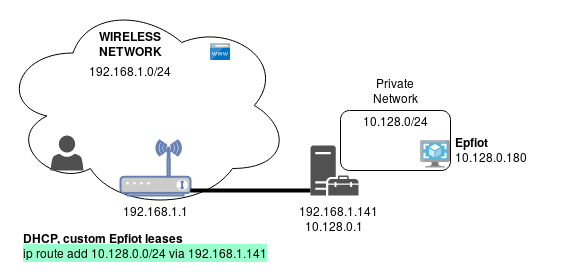
\includegraphics[width=5.5in]{figures/Epfiot_example.png}
~\caption{Epfiot Scenario}
\label{figure6.1}
\end{figure}

\newpage
\section{Authentication and basic use}
\label{makereference6.2}

Epfiot is user based, at the moment there is no public service dedicated to Epfiot and the installation is private.
For the alpha version (current) there are a number of example users already created to be able to test the application. 

The user Charlie@gmail.com has access to the Epfiot alpha and proceeds to enter into the application. Epfiot has an authentication system so you have to enter a username and password if you want to interact.
\begin{figure}[h!]%t=top, b=bottom, h=here
\centering
    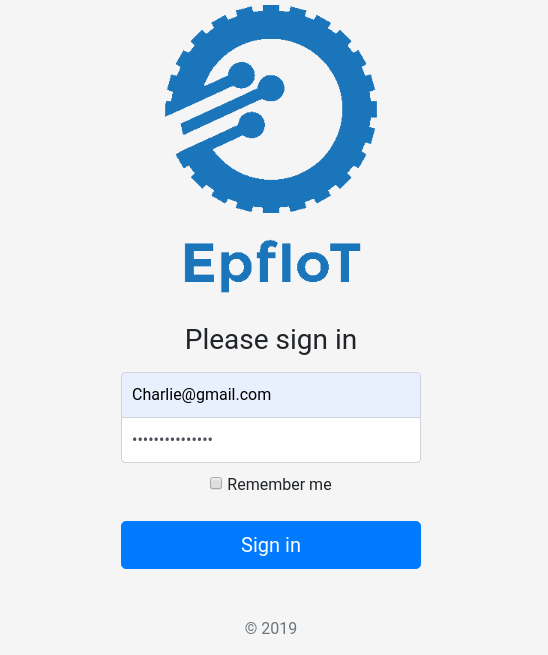
\includegraphics[width=3.5in]{figures/login.png}
~\caption{Epfiot Login}
\label{figure6.2}
\end{figure}

Once inside the application, the alpha version of epfiot provides you with a graphql console.
Charlie can write in this console the operations already seen in Chapter \ref{makereference5}.

This example is a basic use of Epfiot, the user just wants to create a machine in an edge environment.

\newpage
Therefore he will use the createvm operation adding a configuration to be able to enter the machine:

\begin{figure}[h!]%t=top, b=bottom, h=here
\centering
    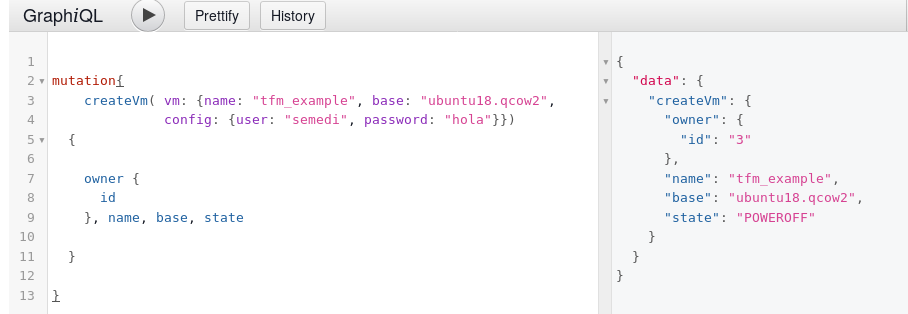
\includegraphics[width=6.5in]{figures/create_vm.png}
~\caption{Vm creation}
\label{figure6.3}
\end{figure}

As you can see, the user is asking for specific return values, such as the status of the machine, its name or even the owner's ID.
When the machine has been created, the user is ready to perform some basic operations like for example turn on the vm:


\noindent\fbox{%
    \parbox{\textwidth}{%
        mutation {
            powerOn(vmID:1){}
        }
    }%
}

Although the command itself gives you a clear feedback on whether the operation has been completed successfully or not, the user probably wants to know more information about his machine. Charlie uses the getvms command to see what is the current status:

\begin{figure}[h!]%t=top, b=bottom, h=here
\centering
    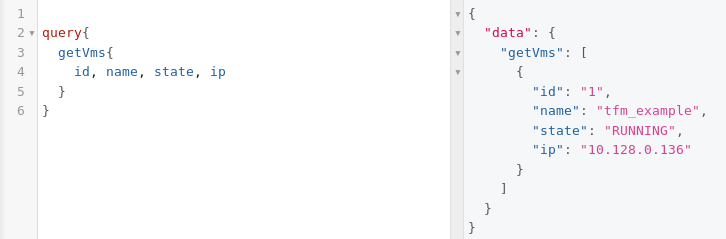
\includegraphics[width=5.5in]{figures/get_vms.png}
~\caption{Vm creation}
\label{figure6.4}
\end{figure}

At this point, Charlie is able to use his new machine in the edge environment.  It is important to note that the machine is accessible through ssh, using as credentials those which are already provided in the creation of the machine. In this example, the user will build everything on his own and only uses Epfiot to create basic infrastructure.

\newpage
\section{Using vms and accelerators}
\label{makereference6.3}

In this example Charlie is going to use one of the most important features of Epfiot as it is to be able to use real hardware accelerators with your machine.

To do this, he's going to use two machines.


\begin{itemize}
    \item The first is the one used in the first example. For this machine (10.128.0.136) Charlie will attach the Google Coral accelerator to test if there is any performance improvement when making inference.
    \item He will create another machine (just like the first example), this time without any device attached. The purpose is to see if there was really a deterioration in the speed compared to the previous test.
\end{itemize}

First of all, Charlie should check with usb devices are available on the host, for this Epfiot has the getusb operation, which gives you a list of the physical devices:
\begin{figure}[h!]%t=top, b=bottom, h=here
\centering
    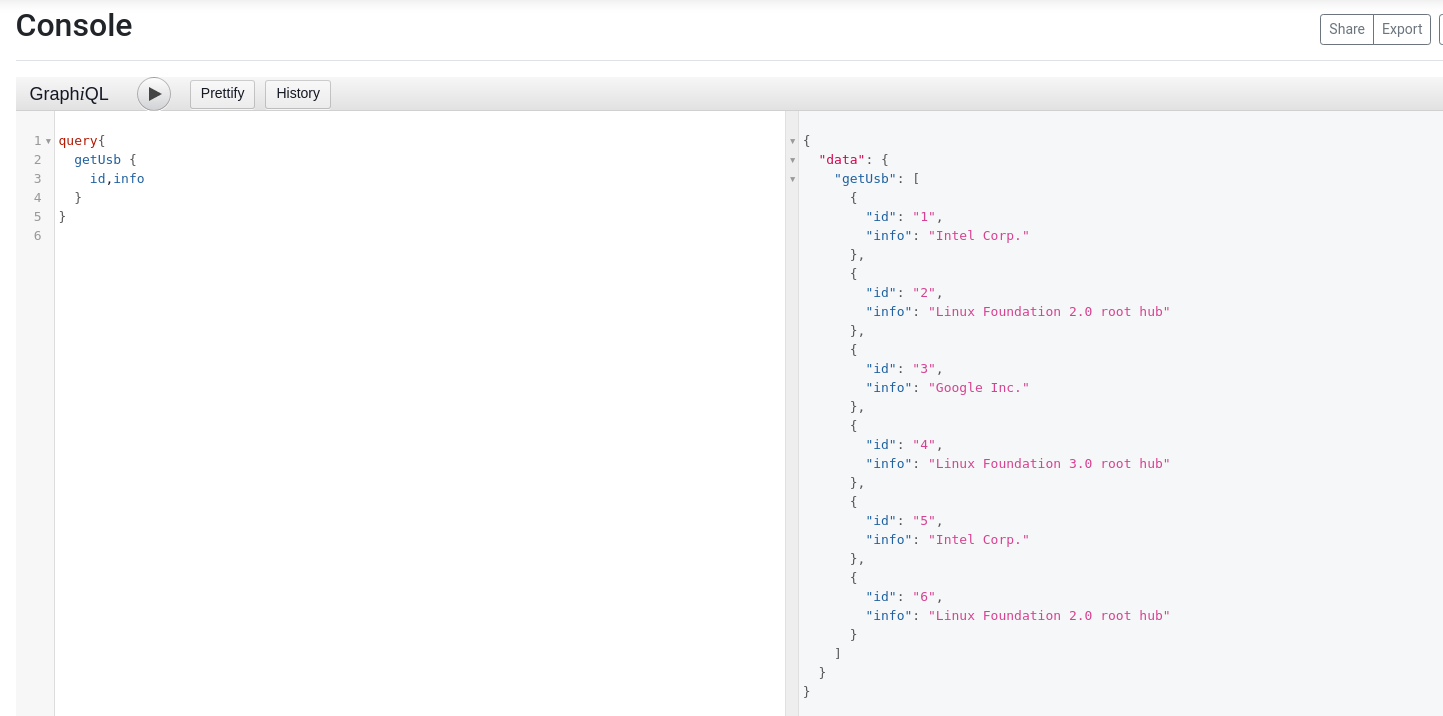
\includegraphics[width=7.0in]{figures/lsusb.png}
~\caption{lsusb operation}
\label{figure6.5}
\end{figure}
\newpage

In this case, we know that Google is the manufacturer of the device, therefore our usb accelerator has de ID 3 as seen in the picture \ref{figure6.5}.

Once we know the device ID, we need to find the ID associated to our machine as well. To do this we can use the \textbf{getVms} operation already done in the figure \ref{figure6.4} where we showed some interesting information of the machine such as the id, status or the ip itself.

If we look at the \textbf{attachDevice} header in Chapter \ref{makereference5.3}, you can see that it needs two arguments which are the IDs already obtained:
\begin{figure}[h!]%t=top, b=bottom, h=here
\centering
    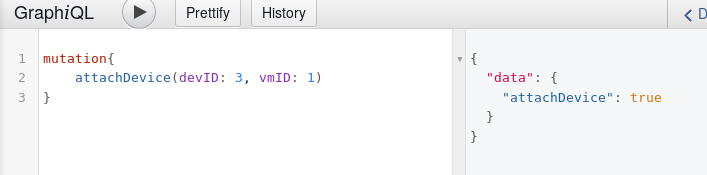
\includegraphics[width=4.5in]{figures/attach_dev.png}
~\caption{attachdevice operation}
\label{figure6.6}
\end{figure}

Epfiot quickly reports that the operation has been successfully completed by returning a boolean value, however Charlie wants to check it himself.
The following image shows the command that Charlie executed on his cmd in order to check that the machine is actually running, it has the user and password indicated by Epfiot and it has a usb accelerator attached:

\begin{figure}[h!]%t=top, b=bottom, h=here
\centering
    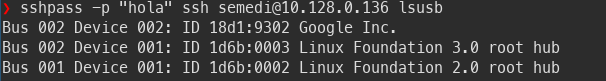
\includegraphics[width=4.5in]{figures/attach_device_ls.png}
~\caption{Charlie checking the machine}
\label{figure6.7}
\end{figure}

As you can see, the machine is operational and has the Google coral installed!

Now that the first machine is ready, Charlie proceeds to create another machine just like the first one, this time without attaching any additional device.
The result is a machine using the Google coral accelerator and another one that will use virtual cpu.
\newpage

\textbf{Using Google Coral Accelerator}

Charlie decides to test if he can really use Google's accelerator from a virtual machine.
To do this, he runs the example code of Google Coral on the machine that has the device attached and gets the following results:

\begin{figure}[h!]%t=top, b=bottom, h=here
\centering
    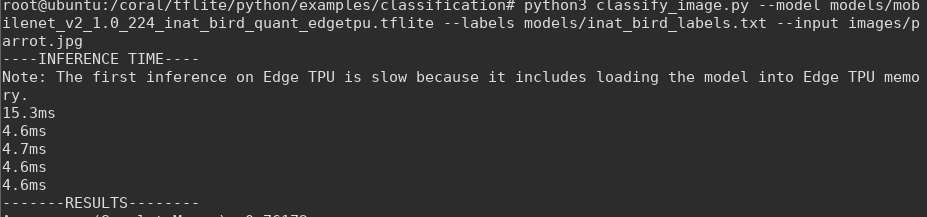
\includegraphics[width=6.5in]{figures/vm_dev_inference.png}
~\caption{Test vm using Google Coral}
\label{figure6.8}
\end{figure}

Charlie gets pretty good results ~4.6ms.

\textbf{Using Virtual Cpu}

Now Charlie is preparing to do the same test using the other machine without the aid of any additional device:

\begin{figure}[h!]%t=top, b=bottom, h=here
\centering
    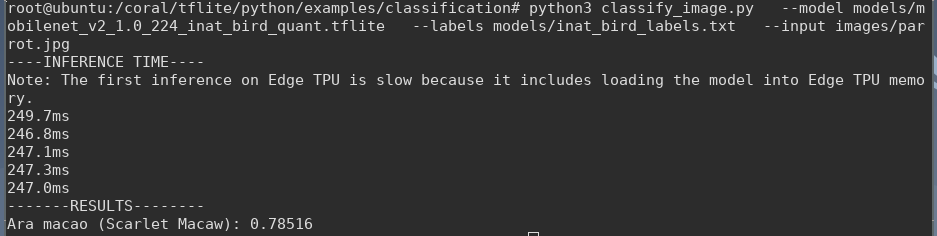
\includegraphics[width=6.5in]{figures/vm_nodev_inference.png}
~\caption{Test vanilla vm}
\label{figure6.9}
\end{figure}

It's easy to see the difference in the results, Charlie gets a speed of ~247ms worsening drastically the results obtained in the previous test.

With this test Charlie has learned that Epfiot's feature of attaching real devices is very useful in certain occasions such as those that could happen in an edge environment.
\newpage
\section{Taking care of things}
\label{makereference6.4}

Once Charlie knows about the real device management feature, he decides to deploy some sensors with which he will build his Internet of Things stack using the infrastructure already created.

For the above test he created two machines, quickly he realizes that he would only need one machine for his stack so he deletes the first one:

\begin{figure}[h!]%t=top, b=bottom, h=here
\centering
    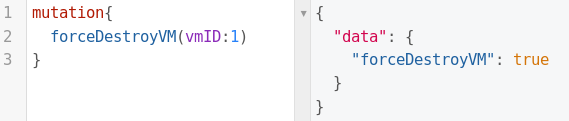
\includegraphics[width=4.5in]{figures/force_destroy.png}
~\caption{destroy a machine}
\label{figure6.10}
\end{figure}

Force destroy operation \ref{makereference5.3} allows you to abruptly remove a machine.

Counting only with one machine, he realizes that he does not remember the given name to the machine. 
For his new test he wants to know the name of the machine, its ip, memory and virtual cpu.

Thanks to graphql, Epfiot allows you to use queries asking only for the desired values:

\begin{figure}[h!]%t=top, b=bottom, h=here
\centering
    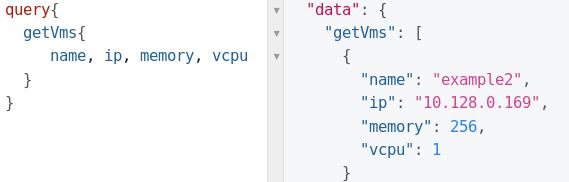
\includegraphics[width=5.5in]{figures/concrete_getvm.png}
~\caption{specific getvm operation}
\label{figure6.11}
\end{figure}

\newpage
Looking at Epfiot's log, he sees that something has happened to the machine. To handle the sensors, Epfiot register the infrastructure on its bootstrapping server. Therefore his "example2" machine is ready to be used with new sensors:

\begin{figure}[h!]%t=top, b=bottom, h=here
\centering
    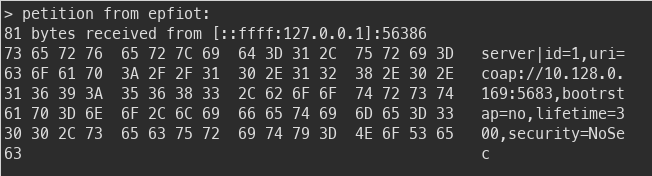
\includegraphics[width=6.5in]{figures/bs_server_log.png}
~\caption{bootstrap server log}
\label{figure6.12}
\end{figure}

This Epfiot functionality allows you to register sensors directly with your infrastructure. Epfiot saves the device information in its bootstrap server, so that as soon as the device enters into the network it can be configured with the setting of the newly created server automatically.
To do this, Charlie creates a new test device on epfiot:

\begin{figure}[h!]%t=top, b=bottom, h=here
\centering
    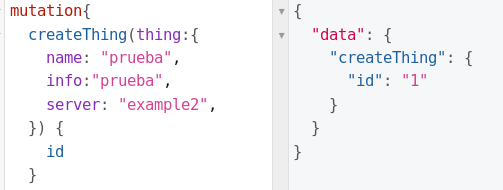
\includegraphics[width=5.5in]{figures/create_thing.png}
~\caption{Create a thing}
\label{figure6.13}
\end{figure}

The "prueba" sensor is now linked to the example2 machine! At least from the point of view of the Epfiot mode (See Figure \ref{figure6.14}).For the device to be automatically configure it must first be deployed on the network where Epfiot is located.

Following the figure \ref{figure6.1}, Charlie deploys his new sensor in the wireless network (192.168.1.0/24). Remember that since the router have a table for 10.128.0.0/24 network, it is possible to access the Epfiot private network and reach the allocated vms.
\newpage

\begin{figure}[h!]%t=top, b=bottom, h=here
\centering
    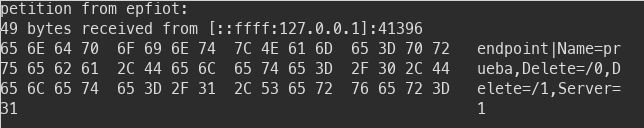
\includegraphics[width=5.5in]{figures/bs_endpoint_log.png}
~\caption{Epfiot bootstrap device registration}
\label{figure6.14}
\end{figure}

With Epfiot ready, Charlie turns on his new lwm2m sensor into the network and watches the generated log:

\begin{figure}[h!]%t=top, b=bottom, h=here
\centering
    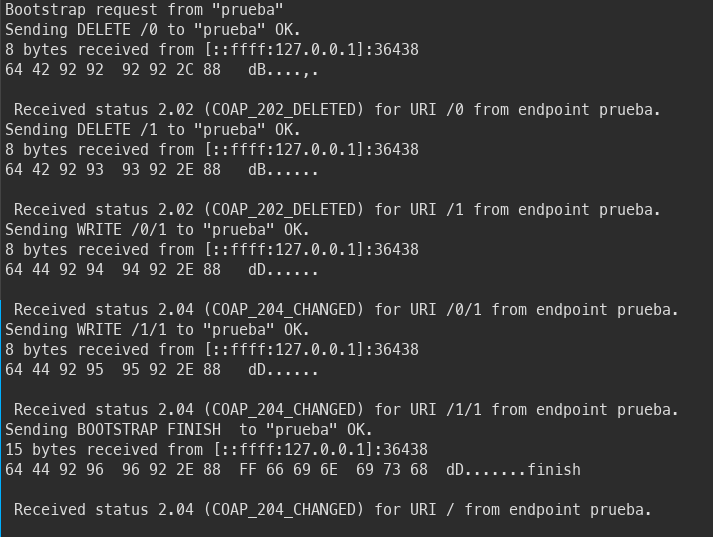
\includegraphics[width=5.5in]{figures/bs_endpoint_log2.png}
~\caption{Epfiot psychical sensor detected}
\label{figure6.15}
\end{figure}

Epfiot discovers this new sensor "prueba" and proceeds to send its new bootstrapping configuration.
In the alpha phase Epfiot follows these steps:
\begin{itemize}
    \item Delete /0 object
    \item Delete /1 object
    \item write the 'master' server configuration (In this case 10.128.0.169).
\end{itemize}
\newpage

To finish his test, Charlie checks if anything has happened on the deployed server, he gets the following results

\begin{figure}[h!]%t=top, b=bottom, h=here
\centering
    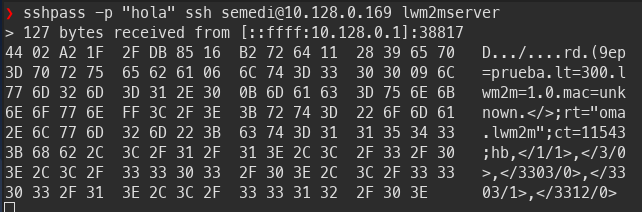
\includegraphics[width=6.5in]{figures/bs_endpoint_log3.png}
~\caption{Deployed vm receiving information about a new device}
\label{figure6.16}
\end{figure}

The "prueba" device is now attached to the virtual machine previously created! All made simple with Epfiot, now from his machine, Charlie can continue to interact remotely with his new sensor.

Since Epfiot has configured the "prueba" sensor, Charlie can also see which devices are active (they are in the network and have been bootstrapped by the application):


\begin{figure}[h!]%t=top, b=bottom, h=here
\centering
    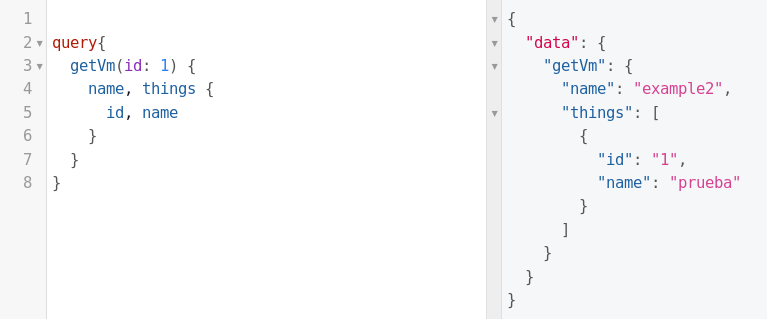
\includegraphics[width=6.5in]{figures/attached_thing.png}
~\caption{The bootstrapped thing}
\label{figure6.17}
\end{figure}
